\documentclass{beamer}

\usepackage[utf8]{inputenc}
\usepackage[spanish]{babel}
\usepackage[outputdir=.build]{minted}
\usepackage{hyperref}
\usepackage{graphicx}
\usepackage{tikz}
\usetikzlibrary{shapes,arrows}

\hypersetup{
    colorlinks = true
}

\usetheme{Madrid}

%Information to be included in the title page:
\title{Taller de Física Computacional}
\subtitle{Condicionales (control de flujo)}
\author{Cristián G. Sánchez y Carlos J. Ruestes}
\date{2020}

\begin{document}

\frame{\titlepage}

%%%%%%%%%%%%%%%%%%%%%%%%%%%%%%%%%%%%%%%%%%%%%%%%%%%%%%%%%%
\begin{frame}[fragile]
    \frametitle{Condicionales}
    \begin{block}{Condicionales}
    Los condicionales son ubicuos en los lenguajes de programación y permiten dividir la ejecución en {\em ramas} distintas
    de acuerdo al resultado de la evaluación de una o más expresiones Booleanas. En Python existen tanto {\bf expresiones} como 
    como {\bf declaraciones} condicionales.
    \end{block}  
    \end{frame}

%%%%%%%%%%%%%%%%%%%%%%%%%%%%%%%%%%%%%%%%%%%%%%%%%%%%%%%%%%
\begin{frame}[fragile]
    \frametitle{Declaraciones y expresiones}
    \begin{block}{Nota}
        El \href{https://docs.python.org/3/reference/index.html}{Manual de Referencia de Python} distingue entre distintos tipos de {\bf expresiones}
        y {\bf declaraciones}. Sin entrar en definiciones estrictas (porque la categorización {\em no es estricta}) podemos decir que:
        \begin{itemize}
            \item Las {\bf expresiones} son combinaciones de elementos sintácticos como identificadores, literales, llamados a funciones,
            operadores, etc. que poseen al menos un \alert{valor}.
            \item Las {\bf declaraciones} se pueden pensar como la mínima unidad imperativa, las declaraciones \alert{hacen algo}. Las asignaciones,
            por ejemplo, son un tipo de declaración. 
        \end{itemize}
    \end{block}    
    \end{frame}
    
%%%%%%%%%%%%%%%%%%%%%%%%%%%%%%%%%%%%%%%%%%%%%%%%%%%%%%%%%%
\begin{frame}[fragile]
    \frametitle{La expresión condicional}
    \begin{block}{La expresión condicional}
    La mínima unidad de código de ejecución condicional en python es la siguiente:
    \begin{minted}{python}
    a = X if Z else Y
    \end{minted}
    donde $Z$ es una variable o expresión Booleana y $X$ e $Y$ son dos variables, expresiones o literales. 
    Si $Z$ es \mintinline{python}{True} la variable $a$ tomará el valor $X$, si es \mintinline{python}{False} 
    tomará el valor $Y$.
    \end{block}
    \end{frame}

%%%%%%%%%%%%%%%%%%%%%%%%%%%%%%%%%%%%%%%%%%%%%%%%%%%%%%%%%%
\begin{frame}[fragile]
    \frametitle{Declaraciones condicionales}
    \begin{block}{La declaración condicional más simple}
    La declaración condicional más simple en python es la siguiente:
    \begin{minted}{python}
    if X: (declaración)
    \end{minted}
    donde \mintinline{python}{(declaración)} es una única línea de código que es ejecutada si la expresión $X$ es \mintinline{python}{True}.
    \end{block}

    \end{frame}

    %%%%%%%%%%%%%%%%%%%%%%%%%%%%%%%%%%%%%%%%%%%%%%%%%%%%%%%%%%
\begin{frame}[fragile]
    \frametitle{Declaraciones condicionales}

    \begin{block}{La declaración condicional}
        La declaración condicional que sigue en complejidad es la siguiente:

        \begin{minted}[showspaces=true,autogobble=true]{python}
    if X: 
        (declaración 1)
        (declaración 2)
        # y sigue...
        \end{minted}

        donde la serie de declaraciones indentadas son ejecutadas si la expresión $X$ es \mintinline{python}{True}. Como vimos en el caso de la
        definición de funciones la \alert{indentación} es una parte fundamental de la estructura.
        \end{block}
    \end{frame}

%%%%%%%%%%%%%%%%%%%%%%%%%%%%%%%%%%%%%%%%%%%%%%%%%%%%%%%%%%%

%%%%%%%%%%%%%%%%%%%%%%%%%%%%%%%%%%%%%%%%%%%%%%%%%%%%%%%%%%
\begin{frame}[fragile]
    \frametitle{Declaraciones condicionales}
    \begin{block}{La declaración condicional}
        La declaración condicional que sigue en complejidad es la siguiente:
        \begin{minted}[showspaces=true,autogobble=true]{python}
    if X: 
        (declaración 1)
        (declaración 2)
        # y sigue...
    else:
        (declaración 1)
        (declaración 2)
        # y sigue...
        \end{minted}
        donde la serie de declaraciones indentadas luego de la línea que contiene al \mintinline{python}{if}
        son ejecutadas si $X$ es \mintinline{python}{True} y si $X$ es \mintinline{python}{False} se ejecutan
        las declaraciones indentadas luego de la línea que contiene al \mintinline{python}{else}.
        \end{block}
    \end{frame}

%%%%%%%%%%%%%%%%%%%%%%%%%%%%%%%%%%%%%%%%%%%%%%%%%%%%%%%%%%

\begin{frame}[fragile]
    \frametitle{La declaración condicional más completa}

\begin{columns}
    \begin{column}{0.5\textwidth}
        \begin{minted}[showspaces=true]{python}
if (condición 1):
    pasar.cosas("esto")
elif (condición 2):
    pasar.cosas("aquello")
elif (condición 3):
    pasar.cosas("lo de más allá")
else:
    pasar.cosas("oops") 
        \end{minted}
    \end{column}
    \begin{column}{0.5\textwidth}
        \begin{center}
            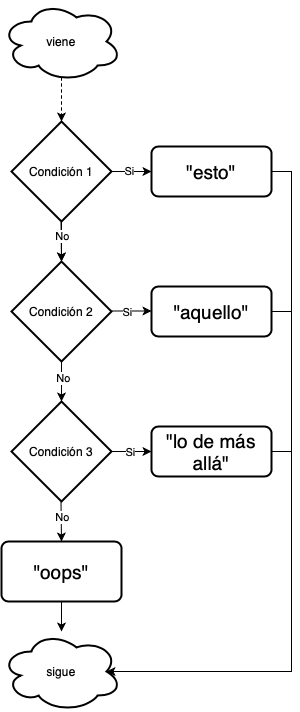
\includegraphics[height=7cm]{figuras/flow.png}           
        \end{center}    
    \end{column}

\end{columns}
 \end{frame}

%%%%%%%%%%%%%%%%%%%%%%%%%%%%%%%%%%%%%%%%%%%%%%%%%%%%%%%%%%

\begin{frame}[fragile]
    \frametitle{Condicionales y eficiencia}

\begin{columns}
    \begin{column}{0.3\textwidth}
        
\includegraphics[width=3cm]{figuras/sin.png}
    \end{column}
    \begin{column}{0.7\textwidth}
        Los condicionales son de extrema utilidad en programación. Sin embargo al causar lo que se denomina {\em branching} (ramificación), tienen una penalidad
        en términos de eficiencia. El {\em branching} hace que el procesador deje de ejecutar una secuencia de instrucciones y deba saltar una secuencia
        diferente de instrucciones. 
    \end{column}

\end{columns}
 \end{frame}

%%%%%%%%%%%%%%%%%%%%%%%%%%%%%%%%%%%%%%%%%%%%%%%%%%%%%%%%%%

\begin{frame}[fragile]
    \frametitle{Condicioneales y eficiencia}

\begin{columns}
    \begin{column}{0.3\textwidth}
        
\includegraphics[width=3cm]{figuras/sin.png}
    \end{column}
    \begin{column}{0.7\textwidth}
        Mucha de la ingeniería de eficiencia en los procesadores modernos se basa en la predictibilidad de un programa. El {\em branching}
        rompe la predictibilidad y por lo tanto disminuye la eficiencia. Los condicionales deben ser evitados particularmente dentro de los bucles,
        en donde se ejecutan, potencialmente, muchísimas veces. De ser posible el código debe ser estructurado para que las declaraciones condicionales
        se ejecuten fuera de los bucles. Las estructuras condicionales dentro del código paralelo imponen también penalidades en términos de eficiencia.
    \end{column}

\end{columns}
 \end{frame}

%%%%%%%%%%%%%%%%%%%%%%%%%%%%%%%%%%%%%%%%%%%%%%%%%%%%%%%%%%%

\begin{frame}
\frametitle{Síntesis y recursos:}

\begin{itemize}
\item \href{https://en.wikipedia.org/wiki/Conditional_(computer_programming)}{Condicionales en Wikipedia}
\item \href{https://docs.python.org/3/reference/index.html}{Manual de Referencia de Python} 

\end{itemize}
\end{frame}

\end{document}
